\documentclass[12pt,a4paper]{article}
\usepackage[english, science, large]{../template/ku-frontpage}
\usepackage{tabularx}
\usepackage{ltablex}
\usepackage{minted}
\setminted[text]{
frame=lines,
framesep=2mm,
baselinestretch=1.1,
fontsize=\footnotesize,
linenos,
breaklines}
\hypersetup{
    colorlinks=false,
    pdfborder={0 0 0},
}
\begin{document}

\title{ACS Theory Assignment 1}
\subtitle{}

\author{Kai Arne S. Myklebust, Silvan Adrian}
\date{Handed in: \today}
	
\maketitle
\tableofcontents

\section{Question 1: Techniques for Performance}
\subsection{Question 1.1}
Concurrency may improve latency, but one must be careful because of locking and correctness. While using concurrency two processes may need to write on the same element and then one process needs to be locked and latency may get worse.
\subsection{Question 1.2}
\textbf{Batching} is when you run multiple requests at once. One example is billing in a credit card company, where they run a monthly billing cycle. All data gets collected at the end of the month and sent at once. \\
\textbf{Dallying} is when you wait until you have some requests accumulated and then run them. One example is where a request comes in too overwrite a disk block, but waits for more requests that may overwrite the same disk block. Then the first request would not be needed anymore. \\
Batching may improve latency and throughput, but dallying typically incurs a latency penalty because it waits for more requests.
\subsection{Question 1.3}
Yes, because it makes one optimized path for common requests, where it tries to eliminate the need for reads and writes in lower level memory. But only goes deeper when needed.

\section{Question 2: Fundamental Abstractions}
\subsection{Question 2.1}
We need some central machine which can translate an address from the single space address into the address for one of the $k$ machines.
On this machine there would be a look up table present, in which we can look up any of the $k$ machine addresses.
The performance for looking up such an address would be done by linear search which could end up very slow with a lot of machines.

The biggest disadvantage is that there is a central lookup machine needed and in case that machine is not available, none of the machines will be reachable.
Sure we could extend the amount of central machines (for example using proxies with caches).
Also in case any machine is shutdown, we would use a time out so that at least request will be handled properly.

\subsection{Question 2.2}

\begin{minted}{text}
write (address, value) {
	k_address = lookup(address)
	try request(k_address)
	catch exception
		throw exception
}

value <- read (address) {
	k_address = lookup(address)
	try request(k_address)
	catch exception
		throw exception
}
\end{minted}

In both read and write we first have to lookup the address we need for sending the request to. We then try to send that request and in case any exception gets thrown we catch it and rethrow it again, so that clients are able to handle those exceptions.

\subsection{Question 2.3}
Yes in regular main memory READ/WRITE operations are atomic.
In our design we do think atomicity is important and we rather what to handle it on the machines side then the client needing to implement additonial code for it.
We can achieve atomicity with a locking mechanism, that would lock further READ requests if a WRITE request is running, for this we would also need to keep the lookup table consistent so that clients know which machine is locked momentarily and which not.

\subsection{Question 2.4}
No the memory locations will get unavailable, since we keep the address in the single address space and only handle it by timeout if a machine is not reachable (or even doesn't exist anymore).
We could extend the lookup table with a possible flag of not existing machines, but the address would still live on in the table which could end up in a table which has many unused addresses in it.
For that we would have to free up some spaces and move addresses back and forth then we would be able to also get rid of puttings too much unneeded data into the lookup table.


\section{Question 3: Serializability \& Locking}

\subsection{Precedence graph}
\subsubsection{Schedule 1}
Yes it is conflict-serializable, because there is no cycle in the precedence graph.
\begin{figure}[!htb]
	\center
	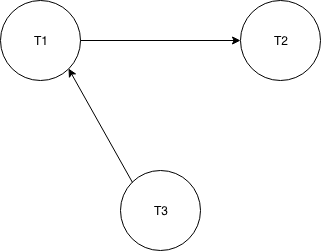
\includegraphics[width=0.5\textwidth]{img/schedule1}
	\caption{Precedence graph of schedule 1}
\end{figure}\\
\subsubsection{Schedule 2}
Yes, since the precedence graph has no precedences and therefore also no cycle.

\subsection{Strict 2PL scheduler}

\subsubsection{Schedule 1}
Transaction 2 has a write on X but there is already a shared lock on X in T1, that's why it has to abort.
\begin{figure}[!htb]
	\center
	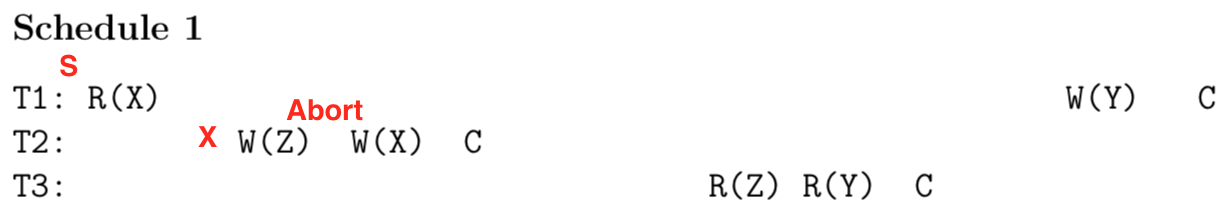
\includegraphics[width=\textwidth]{img/Schedule1_strict2PL}
	\caption{Schedule 1, strict 2PL}
\end{figure}


\subsubsection{Schedule 2}
Yes it can be generated by strict 2PL scheduler, see figure.
\begin{figure}[!htb]
	\center
	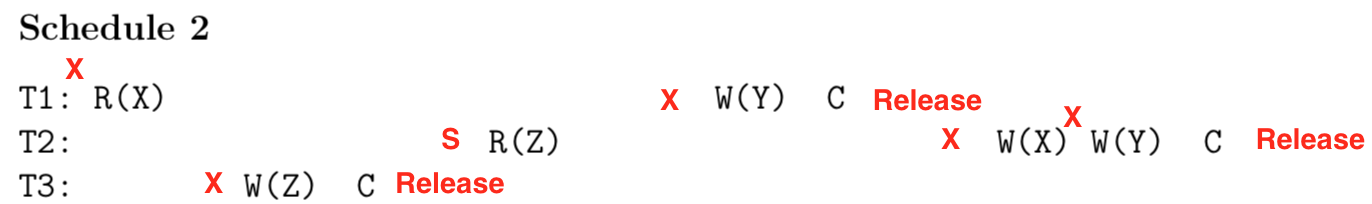
\includegraphics[width=\textwidth]{img/Schedule2_strict2PL}
	\caption{Schedule 2, strict 2PL}
\end{figure}

\section{Question 4: Optimistic Concurrency Control}
\subsection{Scenario 1}
\begin{itemize}
\item T1 completes before T3 starts, so it matches Test 1.
\item T2 does not complete before T3 starts, so it does not match Test 1.
\item T2 completes before T3 begins with its write phase, but the intersection of WriteSet(T2) and ReadSet(T3) is \{4\}. So it is not empty and does not match Test 2.
\item T2 completes its read phase before T3 does, so the second condition in Test 3 is again not empty as in Test 2. So it does not match Test 3.
\end{itemize}
Therefore we roll back.
\subsection{Scenario 2}
\begin{itemize}
\item T1 does not complete before T3 starts, so it does not match Test 1.
\item T1 completes before T3 begins with its write phase, but the intersection of WriteSet(T1) and ReadSet(T3) is \{3\}. So it is not empty and does not match Test 2.
\item T1 completes its read phase before T3 does, so the second condition in Test 3 is again not empty as in Test 2. So it does not match Test 3.
\end{itemize}
T1 did not match any Tests so we do not need to check T2 and we roll back.
\subsection{Scenario 3}
\begin{itemize}
\item T1 does not complete before T3 starts, so it does not match Test 1.
\item T1 completes before T3 begins with its write phase, and the intersection of WriteSet(T1) and ReadSet(T3) is empty. So it matches Test 2.
\item T2 does not complete before T3 starts, so it does not match Test 1.
\item T2 completes before T3 begins with its write phase, and the intersection of WriteSet(T2) and ReadSet(T3) is empty. So it matches Test 2.
\end{itemize}
Both T1 and T2 passed a test, so we can commit.
\end{document}}